\documentclass[12pt]{article}
\usepackage[margin=1in]{geometry}
\usepackage{hyperref}
\usepackage[utf8]{inputenc}
\usepackage{amsmath}
\usepackage{graphicx}
\graphicspath{ {./images/} }
\usepackage{subcaption}
\usepackage{physics}
\setlength{\parskip}{1em}
\usepackage{minted}
\usepackage{xcolor} % to access the named colour LightGray
\definecolor{LightGray}{gray}{0.9}
\usepackage{indentfirst}
\usepackage{url}
\usepackage{wrapfig}
\title{CTA200 Assignment 3}
\author{Isabella Armstrong \\ 1006822967\\
\href{mailto:isabella.armstrong@mail.utoronto.ca}{isabella.armstrong@mail.utoronto.ca}}
\date{\today}
\usepackage{ragged2e}

\begin{document}
\maketitle


\section{Question 1: Mandelbrot Set}
\subsection{Goal of the Section}


In this section we will calculate and plot the Mandelbrot set on the reduced domain domain $D = \{ (x,y)| -2 \leq x\leq 2, -2\leq y\leq2\}$. A Mandelbrot set is defined as the set of complex numbers, $z = x + iy$, which do not diverge to infinity when equation (\ref{eqn:iterate}) is iterated with $z_0 =0 $ \cite{wiki} 
\begin{equation}\label{eqn:iterate}
    z_{i+1} = z^2_i + c
\end{equation}
As equation (\ref{eqn:iterate}) is iterated, some points will remain bounded, as defined by equation (\ref{eqn:bound}), where $Re(z)$ is the real part of $z$ and $Im(z)$ is the imaginary part of z. 
\begin{equation}\label{eqn:bound}
    |z|^2 = Re(z)^2 + Im(z)^2
\end{equation}


\subsection{Methods}

A point was said to diverge when $|z|^2 > 10^{100}$.
To iterate equation (\ref{eqn:iterate}) over the desired domain, a python function was written which took in the value of $Re(z)$,  $Im(z)$, and a maximum number of iterations. The maximum number of iterations was set to 40, which was a reasonable number as most of the divergent points did so in less than 20 iterations. \par 
To iterate over the domain, $D$, two 1D arrays with 300 evenly spaced points within the real and imaginary domain were created. A 2D array of dimensions (x,y) was initialize, and the recursive function applied each cell. The cell was then populated with the number of iterations needed for the point to diverge. If the point did not diverge then the cell was populated with a zero. A total of 90.000 points were tested. \par 

This is seen in figure (\ref{fig:mandelbrot}). The left panel of figure (\ref{fig:mandelbrot}) places a binary condition of the points and the left panels applies a colour grading on the number of iterations needed before divergence. 

\begin{figure}
    \centering
    \begin{subfigure}[h]{0.45\textwidth}
        \centering 
        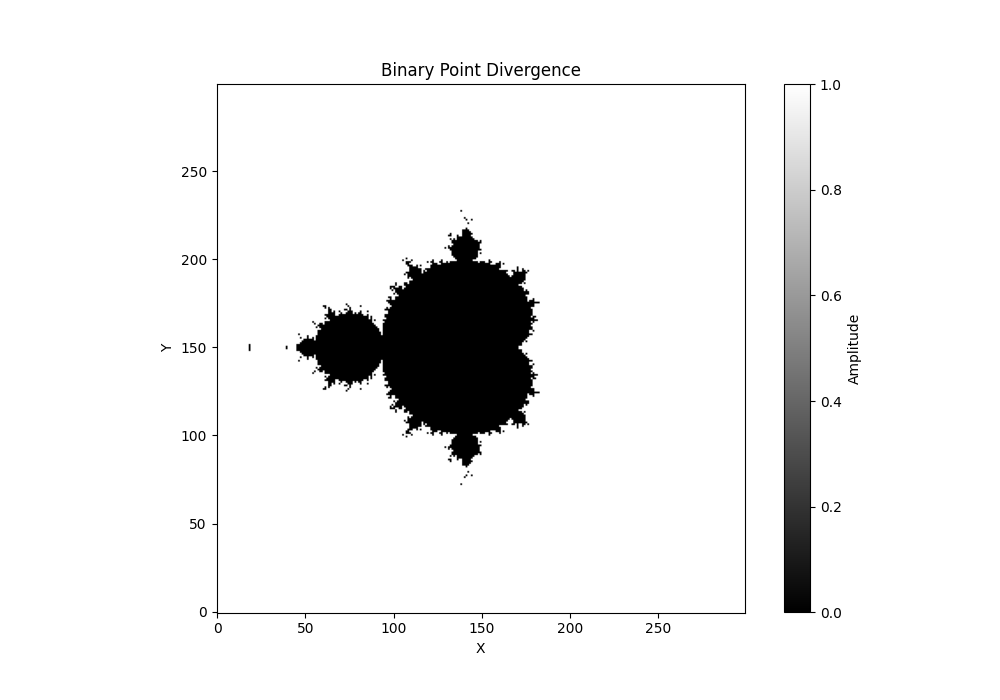
\includegraphics[width=\textwidth]{images/Binary_q1.png}        
    \end{subfigure}
    \begin{subfigure}[h]{0.45\textwidth}
        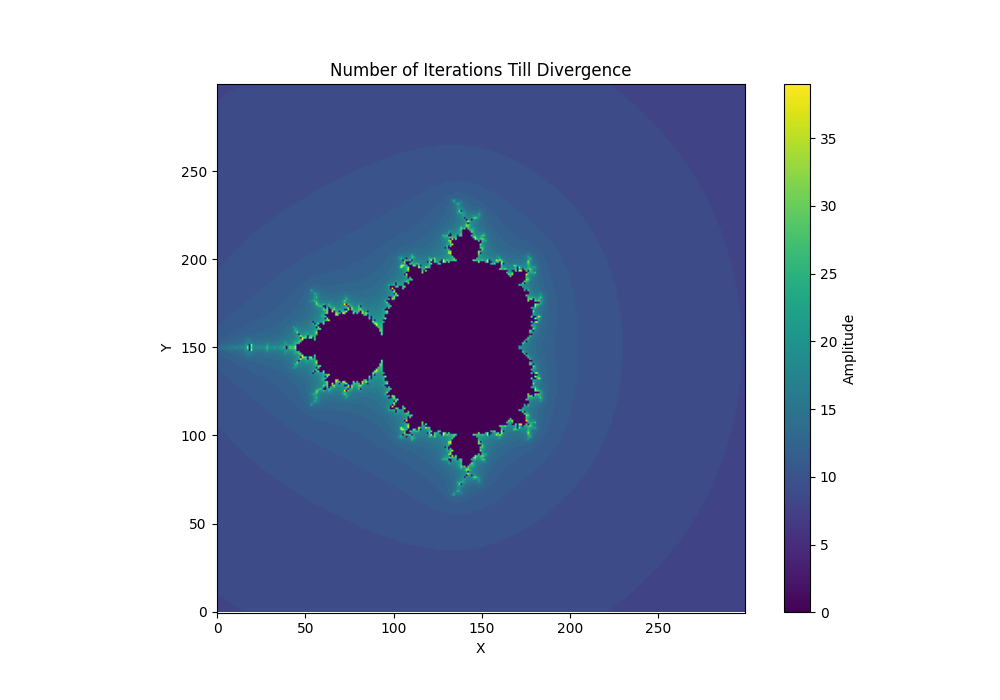
\includegraphics[width=\textwidth]{images/color_Q1.png}
    \end{subfigure}
    \caption{(Left Panel) Binary coding. Points where $|z|^2$ diverges are given in white and points that are bound are given in black. (Right Panel)Number of iterations before divergence. If a point never diverged, its iteration number is set to 0. Both images had a maximum number of 40 iterations.}
    \label{fig:mandelbrot}
\end{figure}


\section{Lorenz Equations}

\subsection{Replication of Results}
In this section we will be recreating figure 1 and 2 from \cite{DeterministicNonperiodicFlow}. This is done by solving the three Lorenz equations (equations 25,26 and 27 in \cite{DeterministicNonperiodicFlow}) and rewritten below. 
\begin{align}\label{eqn:lorenz}
    \dot{X} &= -\sigma(X - Y) \\
    \dot{Y} &= rX - Y  - XZ \\
    \dot{Z} &= -bZ + XY    
\end{align} 
Where $\sigma, r$ and $b$ are dimensionless parameters. These equations were solved using the {\fontfamily{qcr}\selectfont scipy.integrate.solve\textunderscore ivp}. The equations were integrated for 60 seconds in intervals of $\Delta t = 0.01$. Lorenz's initial conditions $W_0 = [0,1,0]$ and parameter values $[\sigma, r, b] = [10, 28, 8/3]$ were used. Figure (\ref{fig:myfig1}) recreates Lorenz's figure 1 and figure (\ref{fig:myfig2}) recreates Lorenz's figure 2.   

\begin{figure}[h]
    \centering
    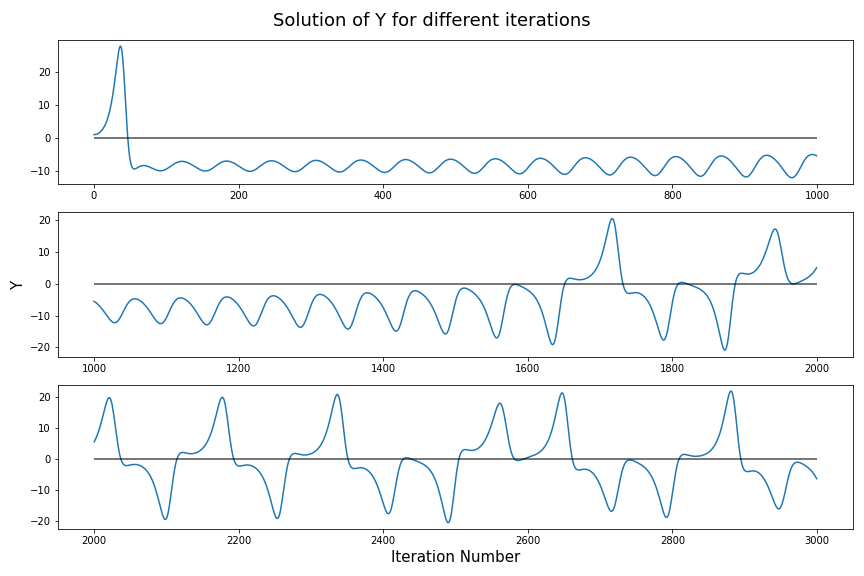
\includegraphics[width=0.8\textwidth]{images/Y_evolution.png}
    \caption{Numerical evolution of Y in the first 1000 (top), 2000 (middle), and 3000 (bottom) Iterations.}
    \label{fig:myfig1}
\end{figure}

\begin{figure}[h]
    \centering
    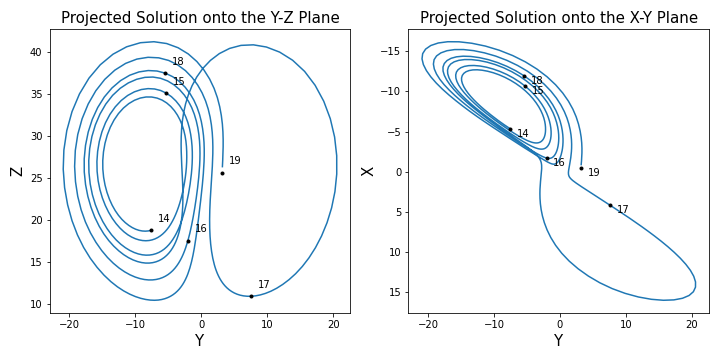
\includegraphics[width=0.9\textwidth]{images/Recreate_fig2.png}
    \caption{Numerical solutions projected into the YZ (left image) and XY (right image) plane for iteration 1400 to 1900. Numbers 14 -19 mark the position, where 14 represents iteration 1400 and so forth.}
    \label{fig:myfig2}
\end{figure}


\subsection{A Small Perturbation}
To see the effect of small perturbations on Lorenz's initial conditions, equations (\ref{eqn:lorenz}) were solved with initial conditions $W' = W_0 + [0, 1e-7, 0]$. The difference between $W'$ and $W_0$ was calculated using equation (\ref{egn:differnce}). Figure (\ref{fig:diverge}) plots this difference as a function of time. It is clear even a small difference in initial conditions leads to exponential growth. Within 40 seconds, the two solutions are two orders of magnitude apart.  
\begin{equation}\label{egn:differnce}
    |W_0 - W'|^2 = (x_0 - x')^2 + (y_0 - y')^2 + (z_0 - z')^2
\end{equation}
\begin{figure}[h]
    \centering
    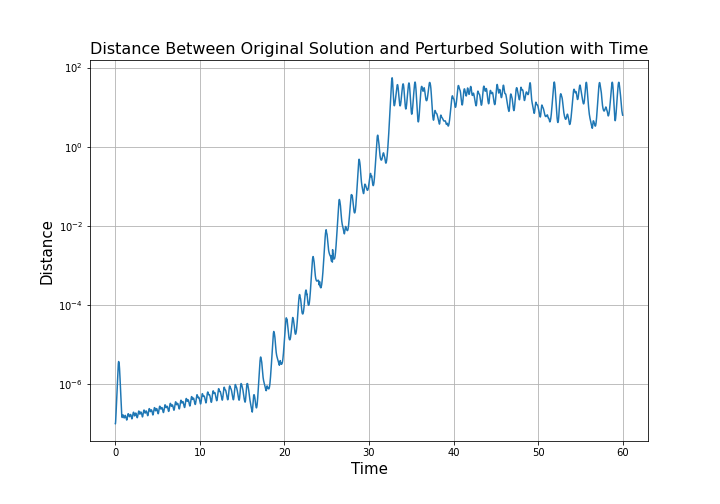
\includegraphics[width=0.9\textwidth]{images/Perturbation.png}
    \caption{The difference between initial condition $W_0$ = [0,1,0] and $W' = [0,1 +1e-7,0]$. It is evident that even a small change initial condition leads to a exponential divergence of solutions. }
    \label{fig:diverge}
\end{figure}

\section{}\label{references}

\bibliographystyle{abbrv}
\bibliography{bib}


\end{document}